\subsection{HA Genghis}

\begin{center}
    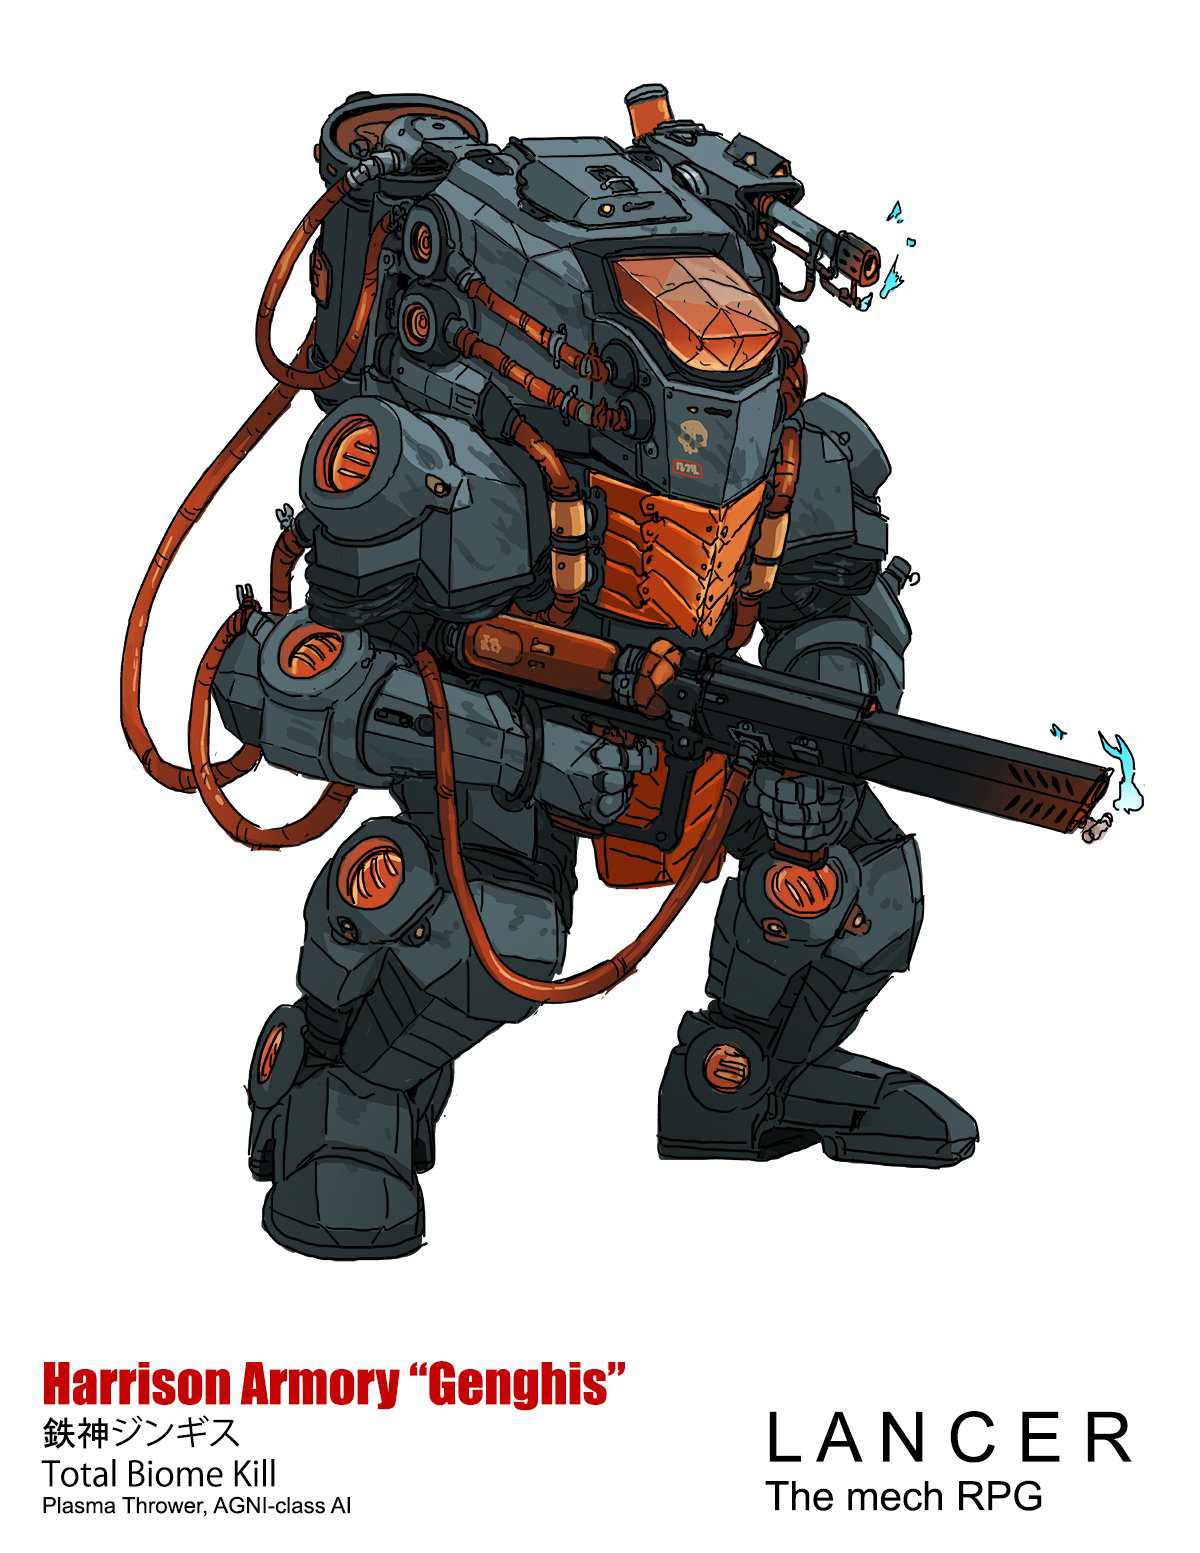
\includegraphics{Genghis}
\end{center}

                                  HARRISON ARMORY GENGHIS

The GENGHIS is a unique Harrison Armory chassis, developed to fill a niche specialist role during the

Hercynia crisis. Due to the unique nature of the Egregorians, a total-biome-kill system was necessary to
ensure localized threat neutralization while keeping Hercynia habitable for future colonists. Thus, the
GENGHIS chassis was developed. Fielding a suite of TBK systems and weapons, GENGHIS squadrons

were dispatched by Union MEF-105 to identify and strike the Egregorian hives. The campaign was a

success, and Hercynia is currently undergoing rehabilitation and repopulation in approved settlement areas.

                                                       License:
I. Flamethrower, Explosive Vent

II. GENGHIS FRAME, Auto-Cooler, HAVOK Mine

III. AGNI Class NHP, Plasma Thrower





                                                GENGHIS

HP: 6          Evasion: 6                            Speed: 3            Heat Cap: 10       Sensors: 5

Armor: 3       E-Defense: 8                          Size: 1             Repair Cap: 4      Tech Attack: -2

                                                  TRAITS:

Insulated: The GENGHIS is immune to Burn

Emergency Vent: When the GENGHIS loses a point of structure, it immediately cools and clears its
heat gauge.

                                            SYSTEM POINTS: 5

                                                 MOUNTS:

Flexible Mount                                        Heavy Mount

                                               CORE system

                                            TBK Sustain Suite
In order to better manage the tremendous power demands of the GENGHIS platform, HA’s Think Tank
developed a suite of power-management protocols to rapidly accelerate heat dispersion. After extensive
field testing, pilots discovered that the TBK Sustain Suite can be tuned to be both a heat sink and a
area-denial weapon.

Active (requires 1 core power): Expose Power Cells
Quick action
You ignore the next overheating check you make this challenge. When you would overheat, clear your
heat from your gauge as normal, but ignore the check (you don’t take stress either). You vent an
enormous cloud of burning matter from your mech, creating a burst 3 area centered on your mech.
Inside the area, all targets (allied and enemy) count as invisible to everyone except you, and all mechs
other than you that enter the area for the first time on their turn or start their turn there take 2 Burn and
2 heat.
On the following round, the benefit from the area reduces to heavy cover (which you ignore). On the
round after that, it reduces to light cover. On the round after that round, the zone disperses.




Flamethrower

The HA Krakatoa was developed specifically for the Hercynian crisis, as chassis-size flamethrowers had

been deemed unnecessary, and more to the point, banned by anti-terror conventions. With the
combination of thick arboreal environment, swarm tactics of the Egregorians, and ineffectual performance
of slug ammunition, the need for a recession on the ban was apparent. The Krakatoa was quickly

developed and affiliate patterns disseminated. Adopted by Union MEF units, the Krakatoa saw heavy use in
the deep world-jungle of Hercynia and towering hives of the Egregorians thanks to its stability, intensity,
and stopping power — a necessary feature competitor makes lacked. Egregorian drones and warriors,

commanded by their overminds, would not stop advancing until they were physically incapable of doing so
— the force at which the Krakatoa expelled flame and fuel was sufficient to knock back or otherwise
incapacitate charging warriors on the periphery of the flame cone. Reworked after the cessation of the

Hercynian crisis, the Krakatoa is now a popular tool for creating area-of-denial firebreaks. It’s legality is
currently under review by the Galactic Treaties Board.

Heavy CQB

Cone 5

Burn 4 + 1 heat


Explosive Vent

Less a technology and more of a tactic, explosive venting is an unsanctioned, unsafe method of sudden
cooling that dumps excess heat into the surrounding area immediately around the chassis.

2 SP, Unique
System




When you cool heat, you explosively vent heat in a burst 1 area around you. Affected targets,
friend or foe, take 1d3 heat and burn.


Auto-Cooler

An HA-designed automatic cooler is a simple, sturdy persistent system that helps pilots mitigate damaging
heat generation.

2 SP, Unique, Protocol
Activate this cooler as a free action at the start of your turn. If you don’t take damage, move, or
overheat before the start of your next turn, cool your mech at the start of your next turn.


HAVOK Mine
FOR USE IN: Urban, post-urban, and high-density terrestrial environments. High O   concentration
                                                                                              2

preferred.

FOR USE AGAINST: Organic targets preferred. Hardened targets vulnerable to caustic/corrosive
degradation preferred. Defoliant. Long-term breach solution.

NOTES: Dispersion is true directional. Dispersion involves aerosolized component -- avoid blue on blue by
supplying end-users with proper respiratory equipment (noted on canister).

2 SP

Mine, Limited (2)
When detonated, this mine attacks a line 5 zone from the mine instead of a burst area around the
mine (oriented in any direction). Affected targets must pass an agility check or take 6 Burn or 3
Burn on a successful check.


Plasma Thrower

The plasma thrower arrived late in the Hercynian Crisis, too late to see widespread battlefield application.
Some MEF squadrons were able to mount the superheavy system, and what little data there is to see from
its use suggests that this system would have had a tremendous impact during the major battles that raged

in the deep jungles during the middle of the Crisis.

Superheavy CQB

4 heat (self)

Cone 7

Burn 5 + 1d6 heat


AGNI-class NHP

AGNI was developed from the aftermath of the Hercynian Crisis using a combination of combat
performance data recorded by extant subsentient artificial intelligences (weapons systems, chassis
copilots, tactic-minds, general combat data) and the neural network of an Egregorian hivemind captured

and vivisected by Union Science Bureau.




Born from trauma, AGNI Prime devised systems of heat management that have since been disseminated
throughout core space to ensure unparalleled heat processing, recycling, and shielding. Further
developments into radiation shielding, omninet capability, and drone/nanite control are forthcoming;

meanwhile, AGNI clones have been optimized for mech chassis core systems.

Pilots report AGNI clones as generally cold and efficient. A low percentage report instances of memory

recitation and command rejection, often followed days later by total breakdown through attempted self-
emancipation. Pilots are recommended to cycle their AGNI clones at least once every six standard months.

3 SP, Unique
AI

Your mech gains the AI property and the AGNI protocol

         AGNI protocol
	        Protocol
         Limited (1)
         At the end of your turn, you automatically cool, clearing your heat gauge. This vent
         creates a burst 3 zone around you. All targets within that zone must make an engineering
         skill check. On a failure, a target takes 2 Burn and is pushed outside the zone (or as far as
         possible). This area provides light cover until the end of your next turn.

         This protocol can only be activated once per scene.
